\documentclass[12pt]{exam}
\usepackage{amsthm}
\usepackage{bm}
\usepackage{libertine}
\usepackage[utf8]{inputenc}
\usepackage[margin=0.5in]{geometry}
\usepackage{amsmath,amssymb}
\usepackage{multicol}
\usepackage[shortlabels]{enumitem}
\usepackage{siunitx}
\usepackage{physics}
\usepackage{booktabs}
\usepackage{graphicx}
\usepackage{pgfplots}
\usepackage{listings}
\usepackage{tikz}
\usepackage{tikz-3dplot}

\bmdefine{\ii}{i}
\bmdefine{\jj}{j}
\bmdefine{\kk}{k}
\newcommand{\te}{\theta}
\newcommand{\cC}{\mathcal{C}}
\newcommand{\word}[1]{\quad\text{#1}\quad}

\pgfplotsset{width=10cm,compat=1.9}
\usepgfplotslibrary{external}
\tikzexternalize
% The existing standalone figures are included directly as PDFs.
\tikzexternaldisable

\newcommand{\class}{Math 261-001}
\newcommand{\examnum}{Quiz 5 Solutions}
% Assumed quiz date: the next weekly Friday after September 29, 2026.
\newcommand{\examdate}{October 2}

\begin{document}
\pagestyle{plain}
\thispagestyle{empty}

\noindent
\textbf{\class}\\
\textbf{\examnum}, \textbf{\examdate}

\vspace{8pt}
\small
\setlength{\abovedisplayskip}{6pt}
\setlength{\belowdisplayskip}{6pt}
\setlength{\abovedisplayshortskip}{3pt}
\setlength{\belowdisplayshortskip}{6pt}
\begin{enumerate}

\item \textbf{Final answer:}
$\boxed{\displaystyle\int_{\pi/4}^{\pi/2}\int_0^{2\cos\theta}r^3\,dr\,d\theta}$.

\smallskip
The Cartesian bounds and the corresponding polar bounds are
\[
  \left\{
  \begin{aligned}
    &0\leq x\leq1,\\
    &x\leq y\leq\sqrt{2x-x^2}
  \end{aligned}
  \right.
  \qquad\Longrightarrow\qquad
  \left\{
  \begin{aligned}
    &\pi/4\leq\theta\leq\pi/2,\\
    &0\leq r\leq2\cos\theta.
  \end{aligned}
  \right.
\]
\begin{minipage}[c]{0.64\linewidth}
\raggedright
The circle is $(x-1)^2+y^2=1$, or $r=2\cos\theta$.
The retained part lies above $y=x$, so its angles run from $\pi/4$
to $\pi/2$. The boundaries meet at $(0,0)$ and $(1,1)$.
These polar bounds also give
$x=r\cos\theta\leq2\cos^2\theta\leq1$.

\medskip
Since $x^2+y^2=r^2$ and $dA=r\,dr\,d\theta$, the transformed
integrand is $r^3$. No evaluation is requested.
\end{minipage}\hfill
\begin{minipage}[c]{0.33\linewidth}
\centering
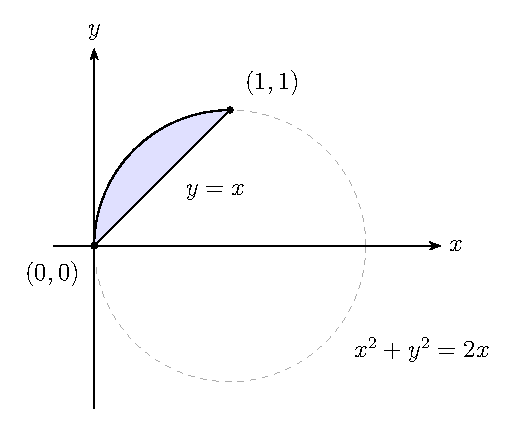
\includegraphics[width=\linewidth]{figures/q5-cartesian-to-polar.pdf}
\end{minipage}

\medskip
\item \textbf{Final answer:} $\boxed{M=4\pi/3}$.

For $-2\leq x\leq-1$, the condition $x^2+y^2\geq1$ is automatic.
The inner circle touches the retained region only at $(-1,0)$.
Thus the Cartesian and polar bounds are
\[
  \left\{
  \begin{aligned}
    &-2\leq x\leq-1,\\
    &-\sqrt{4-x^2}\leq y\leq\sqrt{4-x^2}
  \end{aligned}
  \right.
  \qquad\Longrightarrow\qquad
  \left\{
  \begin{aligned}
    &2\pi/3\leq\theta\leq4\pi/3,\\
    &-\sec\theta\leq r\leq2.
  \end{aligned}
  \right.
\]
\begin{minipage}[c]{0.66\linewidth}
\raggedright
The line $x=-1$ becomes $r\cos\theta=-1$.
Since $\cos\theta<0$ here, dividing $r\cos\theta\leq-1$
reverses the inequality: $r\geq-\sec\theta$.
At $r=2$ the line gives $\cos\theta=-1/2$, determining the
angular endpoints. Also, $-\sec\theta\geq1$ throughout this interval.

\medskip
Multiplying the density $r^2-1$ by the polar area factor $r$ gives
\[
  M=\int_{2\pi/3}^{4\pi/3}\int_{-\sec\theta}^2
  (r^2-1)r\,dr\,d\theta.
\]
\end{minipage}\hfill
\begin{minipage}[c]{0.30\linewidth}
\centering
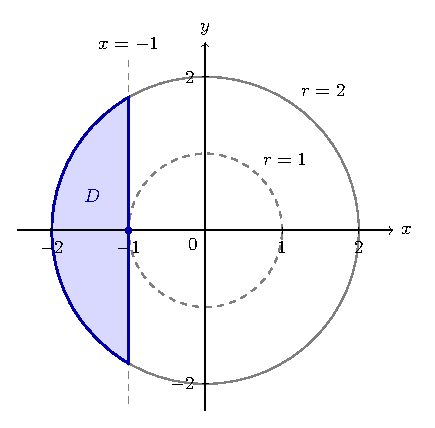
\includegraphics[width=\linewidth]{figures/q5-cut-washer.pdf}
\end{minipage}

Using $\int\sec^4\theta\,d\theta=\tan\theta+\tfrac13\tan^3\theta+C$,
\[
\begin{aligned}
  M&=\int_{2\pi/3}^{4\pi/3}
  \left(2-\tfrac14\sec^4\theta+\tfrac12\sec^2\theta\right)d\theta\\
   &=\left[2\theta+\tfrac14\tan\theta-\tfrac1{12}\tan^3\theta
   \right]_{2\pi/3}^{4\pi/3}=\frac{4\pi}{3}.
\end{aligned}
\]
At either endpoint, $\tan\theta=\pm\sqrt3$, so
$\tfrac14\tan\theta-\tfrac1{12}\tan^3\theta=0$.

\newpage

\item \textbf{Final answer:} the two shaded lobes below, with intersections
$(x,z)=(-2,4),(0,0),(2,4)$.

The given cylindrical bounds and their restriction to $y=0$ are
\[
  \left\{
  \begin{aligned}
    &0\leq\theta\leq2\pi,\\
    &0\leq r\leq2,\\
    &r^2\leq z\leq2r
  \end{aligned}
  \right.
  \qquad\Longrightarrow\qquad
  \left\{
  \begin{aligned}
    &-2\leq x\leq2,\\
    &x^2\leq z\leq2|x|.
  \end{aligned}
  \right.
\]
In Cartesian coordinates the solid satisfies
$x^2+y^2\leq4$ and
$x^2+y^2\leq z\leq2\sqrt{x^2+y^2}$.
On the entire $xz$-plane, $r=\sqrt{x^2}=|x|$.
Consequently, the section has lower boundary $z=x^2$ and upper boundary
$z=2|x|$. Solving $x^2=2|x|$ gives $x=-2,0,2$.

\begin{center}
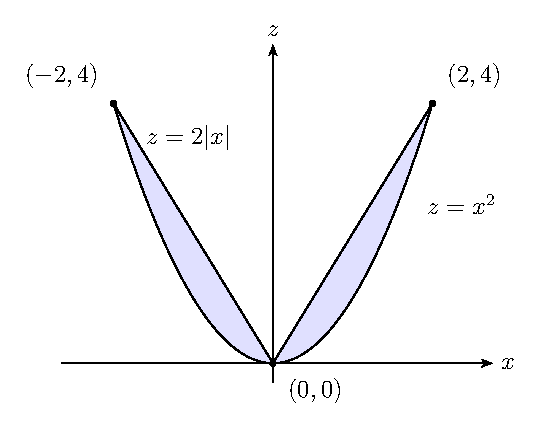
\includegraphics[width=0.50\linewidth]{figures/q5-cone-paraboloid-section.pdf}
\end{center}

% Keep the cross-section diagram and the complete Question 4 solution together.
\newpage
\item \textbf{Final answer:}
\[
  \boxed{\displaystyle
  I=\int_0^1\int_0^z\int_{x^2}^{2x^2}
  z^2x^3e^{x^3}\,dy\,dx\,dz
  =\frac{3-e}{9}.}
\]
Fix a height $z=z_0$, with $0<z_0\leq1$, and view that horizontal plane
in $(x,y)$-coordinates. The first integral covers $R_1$ (blue), and the
second covers $R_2$ (orange):
\begin{center}
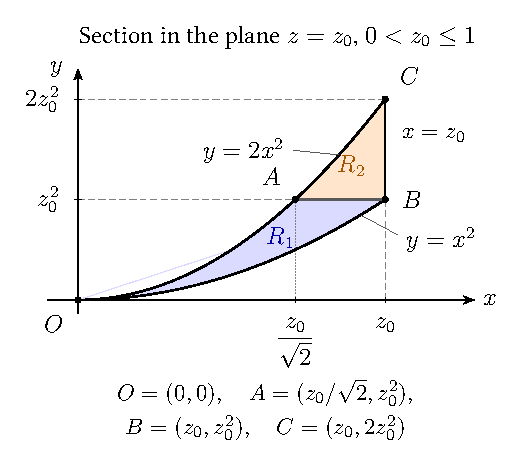
\includegraphics[width=0.62\linewidth]{figures/q5-parabolic-strip-section.pdf}
\end{center}
The pieces share the segment $AB$ on $y=z_0^2$; $BC$ is the boundary
$x=z_0$. The line $y=2z_0^2$ meets the region only at $C$.
The labeled coordinates are $(x,y)$; append $z_0$ to obtain points
in the solid. At $z_0=0$, the section collapses to the origin.

\medskip
For each fixed $0\leq z\leq1$, the two original sections combine as follows:
\[
  \left\{
  \begin{aligned}
    &0\leq y\leq z^2,\\
    &\sqrt{y/2}\leq x\leq\sqrt{y}
  \end{aligned}
  \right.
  \quad\text{or}\quad
  \left\{
  \begin{aligned}
    &z^2\leq y\leq2z^2,\\
    &\sqrt{y/2}\leq x\leq z
  \end{aligned}
  \right.
  \quad\Longleftrightarrow\quad
  \left\{
  \begin{aligned}
    &0\leq x\leq z,\\
    &x^2\leq y\leq2x^2.
  \end{aligned}
  \right.
\]
The curves are $y=x^2$ and $y=2x^2$; the right boundary is $x=z$.
The original upper $x$-bound changes from $\sqrt{y}$ to $z$ at $y=z^2$.
The two pieces meet only along that boundary, so their integrals add
without double-counting volume.

Integrating in $y$ supplies $2x^2-x^2=x^2$. Next use $u=x^3$ and integration
by parts, with $\int ue^u\,du=(u-1)e^u+C$:
\[
\begin{aligned}
  I&=\int_0^1 z^2\int_0^z x^5e^{x^3}\,dx\,dz
    =\frac13\int_0^1 z^2\bigl((z^3-1)e^{z^3}+1\bigr)\,dz\\
   &=\frac19\int_0^1\bigl((v-1)e^v+1\bigr)\,dv
    =\frac19\left[(v-2)e^v+v\right]_0^1
    =\frac{3-e}{9},\qquad v=z^3.
\end{aligned}
\]

\end{enumerate}
\end{document}
